\documentclass[10pt]{article}
\usepackage[margin=1in]{geometry}
\usepackage[T1]{fontenc}
\usepackage{lmodern}
\usepackage{microtype}
\usepackage[hidelinks]{hyperref}
\usepackage{titlesec}
\usepackage{graphicx}
\usepackage{booktabs}
\usepackage{tabularx}
\usepackage{array}
\usepackage{float}
\usepackage[font=small,labelfont=bf]{caption}

\setlength{\parindent}{0pt}
\setlength{\parskip}{0.35em}
\pagestyle{empty}
\titlespacing*{\section}{0pt}{1.2ex plus .2ex minus .2ex}{0.55ex}
\renewcommand{\arraystretch}{1.08}
\captionsetup[figure]{justification=raggedright,singlelinecheck=false,skip=4pt}
\captionsetup[table]{justification=raggedright,singlelinecheck=false,skip=4pt}
\newcolumntype{Y}{>{\raggedright\arraybackslash}X}
\newcolumntype{P}[1]{>{\raggedright\arraybackslash}p{#1}}

\begin{document}

\begin{center}
{\Large\bfseries Role and Callsign Attribution for Flight-Deck Avionics Using Streaming Speaker Diarization and Domain-Tuned ASR\par}
\vspace{0.75em}
{\large Shital Pandey and Jianhua Liu\par}
\vspace{0.2em}
{\normalsize Department of Electrical Engineering and Computer Science\par}
{\normalsize Embry-Riddle Aeronautical University, Daytona Beach, FL, USA\par}
\end{center}
\vspace{0.45em}

\section*{Abstract}

Interpreting air traffic control (ATC) voice communication in real time is essential to flight-deck decision making in the national airspace. An add-on avionics capability for that task therefore needs more than automatic speech recognition (ASR) alone: it must recover who is speaking, whether the transmission comes from a controller or a pilot, and which aircraft callsign the transmission addresses or identifies. This extended abstract presents a role and callsign attribution framework built on streaming speaker diarization and domain-tuned ASR for that purpose. The framework uses streaming Sortformer to estimate local speaker turns and speaker-slot activity, applies a role-attribution layer to label transmissions as controller or pilot, extracts callsign evidence from ASR transcripts, and fuses these signals into structured communication events. By turning ATC voice exchanges into structured events, the system can support instruction/readback awareness on the flight deck while also providing a communication-focused data stream for safety-management and controller-support functions. The completed preliminary foundation comes from verified diarization and role-conditioned analyses on author-revised data derived from the ATC0 dataset. In that foundation, vanilla offline Sortformer reaches 36.6\% diarization error rate (DER) and 14.4\% confusion error rate (CER), calibrated streaming reaches 17.4\% DER and 6.6\% CER, and fine-tuned offline reaches 14.9\% DER and 6.8\% CER. Role-conditioned analysis further shows that controller-side CER reductions exceed pilot-side reductions across all four evaluation recordings. These completed results establish that the current diarization pipeline already provides a feasible front end for avionics-oriented attribution. The planned full paper will add callsign attribution and joint role--callsign evaluation using domain-tuned Whisper transcripts and manually aligned callsign references. Secondary applications include ATC facility review, third-party oversight, and pilot training analysis.

\section*{Motivation and Operational Need}

ATC radiotelephony is central to safe and efficient vehicle operation in the national airspace because operational intent is distributed across short transmissions, multiple speakers, and rapid local turn changes \cite{godfrey1994atcc,wang2024enhancing}. A controller instruction may be followed seconds later by a pilot readback, a correction, or unrelated party-line traffic from another aircraft. A transcript stream by itself is therefore insufficient for a flight-deck aid: without speaker-turn context, role attribution, and callsign identity, it is difficult to distinguish controller-issued instructions from pilot acknowledgements or to identify which aircraft a transmission concerns.

This creates a gap between existing speech technology outputs and operational avionics needs. Prior ATC work has addressed transcription, role-sensitive language understanding, and acoustic diarization \cite{wang2024enhancing,zuluaga2022bertraffic,park2024sortformer,medennikov2025streaming}. However, a usable avionics-support capability requires an intermediate attribution layer that connects local speaker turns, controller/pilot role, and callsign evidence before downstream instruction/readback analysis can be attempted. Structured communication events derived from that layer can support onboard awareness, feed in-time aviation safety management systems (IASMS) through communication and miscommunication monitoring, and provide controllers or related monitoring systems with clearer access to role, callsign, and instruction/readback context. The present abstract focuses on that missing layer.

\section*{Proposed Role and Callsign Attribution Framework}

Figure~\ref{fig:pipeline} summarizes the proposed avionics-support framework. Streaming Sortformer provides the real-time speaker-turn backbone through local activity decisions, turn boundaries, and window-level speaker-slot outputs \cite{park2024sortformer,medennikov2025streaming}. Here, a speaker slot is a local output channel associated with an active speaker inside a short analysis window rather than a persistent identity across an entire recording. In parallel, domain-tuned ASR provides transcript tokens for the same ATC audio.

A lightweight role-attribution layer then labels each transmission or active speaker slot as controller or pilot. This layer can use local acoustic context, slot continuity, and role priors learned from annotation-derived training labels. A callsign-extraction layer operates on the ASR transcript stream to identify addressed or self-identifying callsign mentions. The two outputs are fused into a joint attribution stage that combines role evidence, turn timing, transcript alignment, and callsign evidence to produce a structured event record containing a time interval, active speaker slot, role label, callsign hypothesis, transcript content, and confidence. This event record is the interface to avionics-support functions such as instruction/readback context, communication safety support, and review logging.

\begin{figure}[t]
\centering
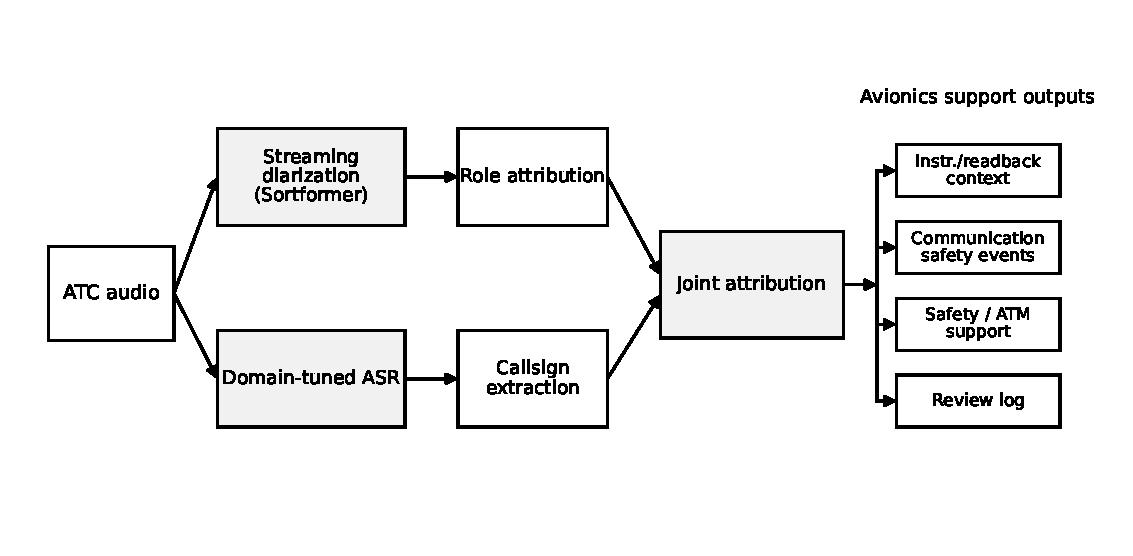
\includegraphics[width=\linewidth]{fig_role_callsign_framework.pdf}
\caption{Proposed role and callsign attribution framework for flight-deck avionics support. Streaming speaker-turn estimation and role attribution operate alongside domain-tuned ASR and callsign extraction, and their outputs are fused into structured communication events.}
\label{fig:pipeline}
\end{figure}

\section*{Preliminary Foundation}

The preliminary foundation for this framework is already substantial. Completed diarization experiments on author-revised data derived from the ATC0 dataset \cite{godfrey1994atcc} show that both calibration and lightweight domain adaptation materially improve segment-level speaker attribution. Table 1 summarizes the verified system-level results. Vanilla offline Sortformer provides the unadapted baseline, vanilla streaming provides the real-time baseline, calibrated streaming demonstrates that threshold transfer can substantially improve the streaming operating point, and fine-tuned offline provides the strongest overall diarization condition in the current package.

The same completed package also contains role-conditioned analysis on the evaluation set. Fine-tuning reduces controller CER by 43.4\% to 66.2\% across the four evaluation recordings, while pilot CER falls by 38.6\% to 49.3\%. Controllers account for 54.5\% to 63.0\% of labeled speech time on those recordings. These results do not yet constitute a role classifier, but they do show that the current streaming and adapted diarization outputs capture distinctions that are meaningful for controller--pilot attribution.

The planned callsign branch will use domain-tuned ASR transcripts aligned to the same ATC audio, consistent with prior ATC speech-recognition studies \cite{wang2024enhancing,radford2022whisper}. In the present abstract, the completed quantitative results remain the diarization and role-conditioned analyses summarized in Table 1.

\begin{table}[H]
\centering
\caption{Verified preliminary foundation from completed diarization and role-conditioned analyses on author-revised data derived from the ATC0 dataset. DER = diarization error rate. CER = confusion error rate.}
\label{tab:foundation}
\begingroup
\footnotesize
\setlength{\tabcolsep}{3.5pt}
\renewcommand{\arraystretch}{1.18}
\begin{tabularx}{\linewidth}{@{}>{\raggedright\arraybackslash\hsize=0.6\hsize\linewidth=\hsize}X>{\raggedright\arraybackslash\hsize=0.9\hsize\linewidth=\hsize}X>{\raggedright\arraybackslash\hsize=1.5\hsize\linewidth=\hsize}X@{}}
\toprule
\textbf{Component} & \textbf{Verified evidence} & \textbf{Monitoring relevance} \\
\midrule
Vanilla offline & 36.6\% DER / 14.4\% CER & Offline baseline for ATC speaker-turn attribution \\
Vanilla streaming & 24.8\% DER / 7.7\% CER & Real-time baseline for local-turn attribution \\
Calibrated streaming & 17.4\% DER / 6.6\% CER & Threshold-transferred streaming condition \\
Fine-tuned offline & 14.9\% DER / 6.8\% CER & Strongest completed diarization condition \\
Role-conditioned analysis & Controller CER reduction 43.4\%--66.2\%; pilot CER reduction 38.6\%--49.3\% & Supports role-sensitive downstream analysis \\
\bottomrule
\end{tabularx}
\endgroup
\end{table}

\section*{Planned Evaluation}

The full paper will evaluate the attribution layer in stages. Table 2 summarizes the planned protocol. The first stage evaluates role attribution at the transmission or active-slot level against controller/pilot labels derived from Segment Time Marked (STM) annotations. The second stage evaluates callsign extraction from domain-tuned ASR transcripts against manually aligned callsign references. The third stage evaluates joint role--callsign attribution and asks whether controller-issued instructions and pilot readbacks can be paired reliably enough to support monitoring-oriented review.

This evaluation moves beyond DER or word error rate alone. The focus is on role F1 score, callsign F1 score, joint attribution accuracy, instruction/readback pairing precision and recall, and targeted error analysis on dense turn regions, party-line traffic, and ambiguous callsign contexts. By framing evaluation around attributed communication events rather than transcript quality alone, the proposed study targets the actual information needed for ATC monitoring.

\begin{table}[H]
\centering
\caption{Planned full-paper evaluation protocol for the attribution layer.}
\label{tab:plan}
\begingroup
\footnotesize
\setlength{\tabcolsep}{3pt}
\renewcommand{\arraystretch}{1.16}
\begin{tabularx}{\linewidth}{@{}>{\raggedright\arraybackslash\hsize=0.8\hsize\linewidth=\hsize}X>{\raggedright\arraybackslash\hsize=1.3\hsize\linewidth=\hsize}X>{\raggedright\arraybackslash\hsize=1.0\hsize\linewidth=\hsize}X>{\raggedright\arraybackslash\hsize=0.8\hsize\linewidth=\hsize}X>{\raggedright\arraybackslash\hsize=1.1\hsize\linewidth=\hsize}X@{}}
\toprule
\textbf{Task} & \textbf{Inputs} & \textbf{Reference / label} & \textbf{Metrics} & \textbf{Purpose} \\
\midrule
Role attribution & Streaming turns, slot activity, and local context & STM-derived role labels & Precision, recall, F1 & Assign controller/pilot role \\
Callsign extraction & ASR tokens aligned to transmission windows & Aligned callsign references & Precision, recall, F1, latency & Recover callsign mentions \\
Joint role--callsign attribution & Role scores, turn timing, transcript alignment, and callsign evidence & Joint transmission labels & Joint accuracy, calibration & Build attributed events \\
Readback pairing & Joint attribution outputs and transcript content & Reviewed instruction/readback pairs & Precision, recall, latency & Support mismatch-oriented review \\
\bottomrule
\end{tabularx}
\endgroup
\end{table}

\section*{Expected Contributions}

This work is expected to make four contributions. First, it introduces an avionics attribution layer that connects streaming diarization and domain-tuned ASR for ATC voice interpretation. Second, it defines a structured communication-event representation that links role, callsign, transcript, and instruction/readback context. Third, it proposes an evaluation protocol that extends beyond DER and transcript quality to role F1, callsign F1, joint attribution accuracy, and communication-monitoring support. Fourth, it provides a preliminary demonstration that the completed streaming diarization and role-conditioned analyses already offer a feasible foundation for a flight-deck aid that interprets ATC voice traffic. Together, these contributions position role and callsign attribution as an enabling layer for avionics that interpret ATC voice traffic, while also producing structured communication evidence useful for safety monitoring, controller support, and post-operation review.

\begingroup
\small
\begin{thebibliography}{00}
\bibitem{godfrey1994atcc}
J. J. Godfrey, \emph{Air Traffic Control Complete LDC94S14A}. Philadelphia, PA: Linguistic Data Consortium, 1994. doi: 10.35111/2bg6-nn53. [Online]. Available: \url{https://catalog.ldc.upenn.edu/LDC94S14A}

\bibitem{wang2024enhancing}
Z. Wang, P. Jiang, Z. Wang, B. Han, H. Liang, Y. Ai, and W. Pan, ``Enhancing Air Traffic Control Communication Systems with Integrated Automatic Speech Recognition: Models, Applications and Performance Evaluation,'' \emph{Sensors}, vol. 24, no. 14, p. 4715, 2024, doi: 10.3390/s24144715.

\bibitem{park2024sortformer}
T. Park \emph{et al.}, ``Sortformer: A Novel Approach for Permutation-Resolved Speaker Supervision in Speech-to-Text Systems,'' in \emph{Proceedings of the 42nd International Conference on Machine Learning}, vol. 267, \emph{Proceedings of Machine Learning Research}, 2025, pp. 48153--48169. [Online]. Available: \url{https://proceedings.mlr.press/v267/park25h.html}

\bibitem{medennikov2025streaming}
I. Medennikov \emph{et al.}, ``Streaming Sortformer: Speaker Cache-Based Online Speaker Diarization with Arrival-Time Ordering,'' in \emph{Proc. Interspeech}, 2025, pp. 5238--5242, doi: 10.21437/Interspeech.2025-2244.

\bibitem{zuluaga2022bertraffic}
J. Zuluaga-Gomez \emph{et al.}, ``BERTraffic: BERT-Based Joint Speaker Role and Speaker Change Detection for Air Traffic Control Communications,'' in \emph{2022 IEEE Spoken Language Technology Workshop (SLT)}, 2023, pp. 633--640, doi: 10.1109/SLT54892.2023.10022718.

\bibitem{radford2022whisper}
A. Radford, J. W. Kim, T. Xu, G. Brockman, C. McLeavey, and I. Sutskever, ``Robust Speech Recognition via Large-Scale Weak Supervision,'' arXiv:2212.04356, 2022. [Online]. Available: \url{https://arxiv.org/abs/2212.04356}
\end{thebibliography}
\endgroup

\end{document}
